\documentclass{article}

\usepackage{graphicx}
\usepackage{tikz}
\usepackage{tikzsymbols}
\usetikzlibrary{calc,patterns,shapes.geometric}
\pagestyle{empty}
\usepackage[margin=0pt]{geometry}
\geometry{papersize={14in,12in}}

\def\centerarc[#1](#2)(#3:#4:#5){\draw[#1] ($(#2)+({#5*cos(#3)},{#5*sin(#3)})$) arc (#3:#4:#5);}

\begin{document}
	\begin{figure}
		\centering
		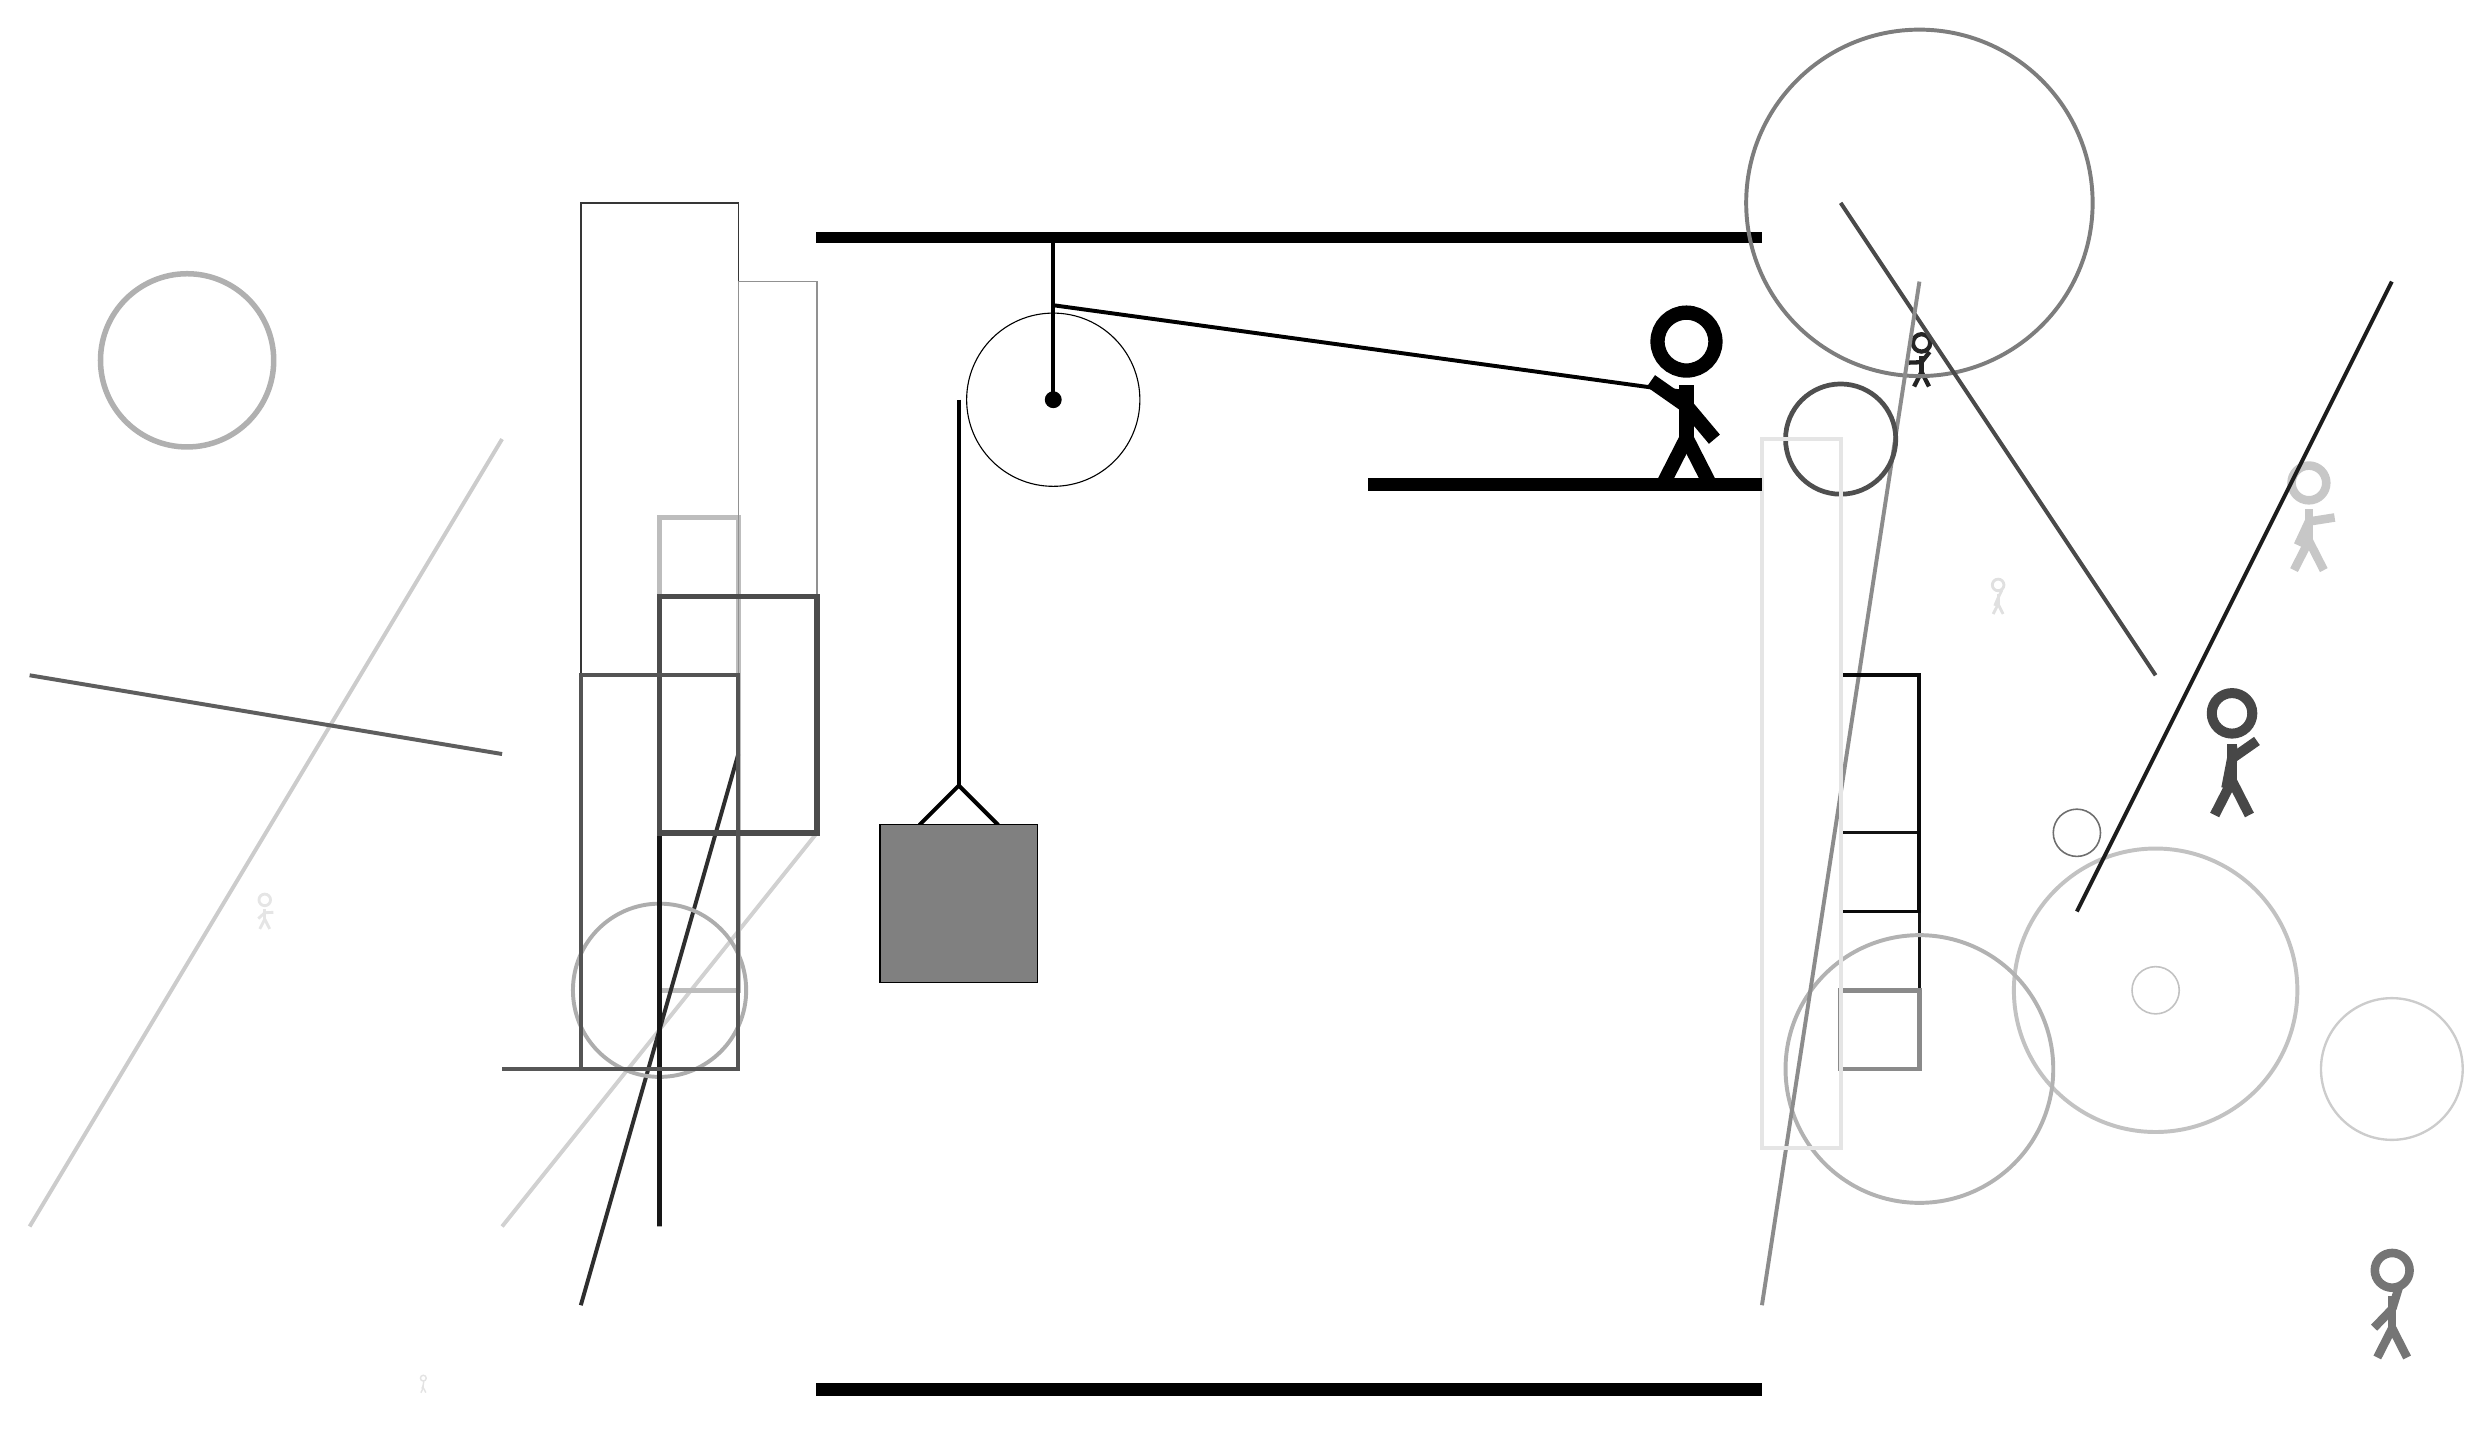
\begin{tikzpicture}
			%%%%% START %%%%%
			
			\draw[fill=black] (-2, 11.5) rectangle (10, 11.625);
			
			\draw (1, 9.5) circle (1.1);
			\draw[fill=black] (1, 9.5) circle (0.1);
			\draw[line width=0.5mm] (1, 11.5) -- (1, 9.5);
			
			\draw[line width=0.5mm, color=black!18](-6, -1) -- (-2, 4);
			
			\draw[line width=0.4mm, color=black!92] (12, 4) rectangle (11, 1);
			\node[line width=0.6mm, color=black!25] at (16, 5) {\Strichmaxerl[1][72][50]};
			\draw[line width=0.6mm, color=black!26] (-3, 2) rectangle (-4, 8);
			\draw [line width=0.5mm, color=black!24](15, 2) circle (1.8);
			\draw[line width=0.5mm, color=black!66](-4, 1) -- (-6, 1);
			\node[line width=0.7mm, color=black!86] at (12, 10) {\Strichmaxerl[3][2][52]};
			\node[line width=0.6mm, color=black!11] at (-7, -3) {\Strichmaxerl[1][71][84]};
			\draw [line width=0.5mm, color=black!51](12, 12) circle (2.2);
			
			\draw[line width=0.5mm, color=black!71](15, 6) -- (11, 12);
			\draw[line width=0.2mm, color=black!79] (-3, 1) rectangle (-5, 12);
			\node[line width=0.6mm, color=black!12] at (13, 7) {\Strichmaxerl[2][67][64]};
			\draw [line width=0.3mm, color=black!20](18, 1) circle (0.9);
			\node[line width=0.6mm, color=black!72] at (16, 5) {\Strichmaxerl[7][79][35]};
			\draw [line width=0.5mm, color=black!30](12, 1) circle (1.7);
			\draw[line width=0.5mm, color=black!20](-6, 9) -- (-12, -1);
			\node[line width=0.2mm, color=black!22] at (17, 8) {\Strichmaxerl[6][65][9]};
			\draw[line width=0.5mm, color=black!82](-5, -2) -- (-3, 5);
			\draw [line width=0.5mm, color=black!32](-4, 2) circle (1.1);
			
			\draw [line width=0.2mm, color=black!57](14, 4) circle (0.3);
			\draw [line width=0.2mm, color=black!24](15, 2) circle (0.3);
			
			\node[line width=0.2mm, color=black!10] at (-9, 3) {\Strichmaxerl[2][42][3]};
			\draw[line width=0.5mm, color=black!89](14, 3) -- (18, 11);
			\draw[line width=0.6mm, color=black!46] (12, 2) rectangle (11, 1);
			\draw[line width=0.5mm, color=black!45](12, 11) -- (10, -2);
			\draw[line width=0.5mm, color=black!54](14, 4) -- (14, 4);
			\draw [line width=0.7mm, color=black!31](-10, 10) circle (1.1);
			\draw [line width=0.6mm, color=black!69](11, 9) circle (0.7);
			\draw[line width=0.5mm, color=black!96] (12, 3) rectangle (11, 6);
			\draw[line width=0.5mm, color=black!63](-6, 5) -- (-12, 6);
			\draw[line width=0.5mm, color=black!10] (11, 0) rectangle (10, 9);
			
			\draw[line width=0.7mm, color=black!91] (-4, -1) rectangle (-4, 4);
			\draw[line width=0.2mm, color=black!43] (-2, 4) rectangle (-3, 11);
			
			\node[line width=0.3mm, color=black!54] at (18, -2) {\Strichmaxerl[6][46][73]};
			
			\draw[line width=0.7mm, color=black!70] (-2, 7) rectangle (-4, 4);
			\draw[line width=0.5mm, color=black!67] (-3, 1) rectangle (-5, 6);
			
			\draw[line width=0.5mm](-0.7, 4.1) --  (-0.2, 4.6) -- (0.3, 4.1);
			\draw[fill=black!50] (-1.2, 4.1) rectangle (0.8, 2.1);
			
			\draw[line width=0.5mm](-0.2, 9.5) -- (-0.2, 4.6);
			\centerarc[line width=0.5mm](1, 9.5)(90:180:1.2000000000000002)
			\draw[line width=0.5mm](1, 10.7) -- (9, 9.6);
			
			\node at (9, 9.5) {\Strichmaxerl[10][-35][-50]};
			\draw[fill=black] (5, 8.5) rectangle (10, 8.35);
			
			\draw[fill=black] (-2, -3) rectangle (10, -3.15);
			
			%%%%% END %%%%%
		\end{tikzpicture}
	\end{figure}	
\end{document}